\documentclass[UTF8,a4paper,12pt]{ctexart}

\usepackage{geometry}
\usepackage{setspace}
\usepackage{graphicx}
\usepackage{booktabs}
\usepackage{tabularx}
\usepackage{array}
\usepackage{xcolor}
\usepackage{caption}
\usepackage{enumitem}
\usepackage{fancyhdr}
\usepackage{hyperref}
\usepackage{url}
\usepackage{float}
\usepackage{listings}

\geometry{top=2.6cm,bottom=2.6cm,left=3.0cm,right=3.0cm}
\setCJKmainfont[BoldFont=SimHei]{SimSun}
\setCJKsansfont{SimHei}
\setmainfont{Times New Roman}
\newCJKfontfamily\coverfont{STLiti}
\linespread{1.35}
\setlength{\parindent}{2em}
\setlength{\parskip}{0.25em}
\setlength{\headheight}{15pt}
\renewcommand{\arraystretch}{1.25}

\definecolor{seublue}{HTML}{1F4D78}
\definecolor{lightblue}{HTML}{F4F6F9}
\hypersetup{
  colorlinks=true,
  linkcolor=seublue,
  urlcolor=seublue,
  citecolor=seublue,
  pdfauthor={课程报告},
  pdftitle={从视觉基础模型到世界模型：2023—2026年计算机视觉算法与技术最新进展综述}
}
\captionsetup{font=small,labelfont=bf}
\setlist[itemize]{leftmargin=2em,itemsep=0.15em,topsep=0.2em}

\pagestyle{fancy}
\fancyhf{}
\fancyhead[C]{\small 从视觉基础模型到世界模型：计算机视觉算法与技术最新进展综述}
\fancyfoot[C]{\small \thepage}
\renewcommand{\headrulewidth}{0.4pt}

\newcolumntype{Y}{>{\raggedright\arraybackslash}X}
\newcolumntype{C}[1]{>{\centering\arraybackslash}p{#1}}
\newcommand{\model}[1]{\textsf{#1}}
\lstdefinestyle{cvpython}{
  language=Python,
  basicstyle=\ttfamily\small,
  keywordstyle=\color{seublue}\bfseries,
  commentstyle=\color{gray},
  stringstyle=\color{teal!70!black},
  numbers=left,
  numberstyle=\tiny\color{gray},
  breaklines=true,
  frame=single,
  rulecolor=\color{lightblue},
  columns=fullflexible,
  tabsize=2,
  showstringspaces=false
}
\lstset{style=cvpython}

\begin{document}

\begin{titlepage}
  \thispagestyle{empty}
  \begin{center}
    
\includegraphics[width=14.5cm]{seu_cover_header.png}
    \vspace{0.35cm}

    {\coverfont\zihao{1} 计算机视觉基础\par}
    \vspace{0.55cm}
    {\coverfont\zihao{1} 课程实验报告\par}
    \vspace{1.5cm}
    {\heiti\zihao{3} 从视觉基础模型到世界模型：\par}
    \vspace{0.25cm}
    {\heiti\zihao{3} 2023—2026年计算机视觉算法与技术最新进展综述\par}
  \end{center}
  \vspace{1.4cm}
  \begin{center}
  \begin{tabular}{C{3.2cm}p{9.2cm}}
    \toprule
    \textbf{题目} & 介绍算法与技术的最新进展 \\
    \midrule
    \textbf{专业} & 英语+信息工程专业 \\
    \textbf{组员} & — @leowrs \\
     & — 组员A \\
    \textbf{任课教师} & 陆建 \\
    \bottomrule
  \end{tabular}
  \end{center}
  \vfill
  \begin{center}
    {\large 主题选择：介绍算法与技术的最新进展（含思政内容）}
  \end{center}
\end{titlepage}

\pagenumbering{Roman}
\section*{摘要}
2023年以来，计算机视觉的主线已经从单一任务模型转向视觉基础模型、视觉语言模型、生成式视频模型、三维几何模型和具身智能模型的融合演进。以\model{DINOv2}、\model{SAM 2}、\model{Florence-2}为代表的视觉基础模型，通过大规模自监督学习、提示式交互和统一任务表示，使检测、分割、描述和跟踪不再完全依赖“一个任务训练一个模型”的范式。以\model{Qwen2.5-VL}、\model{Gemini 1.5}、\model{GPT-4o}和\model{LLaVA-OneVision}为代表的视觉语言模型，把图像、文档、视频、音频和文本纳入统一推理框架，动态分辨率、超长上下文和多模态指令遵循成为新的能力核心。与此同时，\model{Stable Diffusion 3}、\model{Sora}、\model{Movie Gen}等模型推动视觉生成从静态图像走向长视频、音画同步和可编辑媒体；\model{3D Gaussian Splatting}、\model{pixelSplat}、\model{VGGT}等技术则把实时三维重建、多视图几何和可交互场景表示推向应用前沿。更进一步，\model{OpenVLA}、$\pi_0$和\model{V-JEPA 2}显示出视觉模型正在从“看懂”走向“预测、规划和行动”。本文围绕上述技术路线，分析最新算法机制、代表模型、应用价值与风险挑战，并补充一个可复现的小型实验，用RANSAC单应矩阵配准和扰动鲁棒性指标展示“课程基础—前沿模型—评价闭环”的联系。最后，报告结合人工智能治理、科技自立自强和智能向善等要求，讨论计算机视觉发展应坚持的价值导向。

\noindent\textbf{关键词（关键字）：}计算机视觉；视觉基础模型；视觉语言模型；生成式视频；三维重建；具身智能；人工智能治理

\newpage
\tableofcontents
\newpage

\section*{小组分工}
\addcontentsline{toc}{section}{小组分工}
\begin{table}[h]
\centering
\begin{tabularx}{\textwidth}{C{3.5cm}Y}
\toprule
\textbf{成员} & \textbf{主要分工} \\
\midrule
— @leowrs & 承担50\%工作量：资料检索、论文阅读、视觉基础模型与视觉语言模型部分整理、正文撰写与终稿校对。 \\
— 组员A & 承担50\%工作量：生成式视觉、三维视觉与具身智能部分整理、图表制作、参考文献核对与格式检查。 \\
\bottomrule
\end{tabularx}
\end{table}

\newpage
\pagenumbering{arabic}

\section{引言}
传统计算机视觉课程通常从图像滤波、边缘检测、特征匹配、相机标定和图像配准讲起。这些内容构成了视觉系统的几何与信号处理基础：图像如何被采样，像素如何被增强，多个视角如何对齐，三维信息如何从二维投影中恢复。但近三年的研究表明，视觉技术的前沿已经发生明显转向：模型不再只学习某个封闭任务的判别边界，而是通过海量图像、视频、文本和交互数据学习通用表征，并用提示、语言或动作把能力迁移到新任务中。

因此，讨论“算法与技术的最新进展”不能只列举若干模型排行榜。更重要的问题是：这些模型为什么能统一多种视觉任务？视觉语言模型如何突破固定分辨率和短上下文限制？生成式视频为什么被称为世界模拟器？三维重建和具身智能又如何把视觉从识别系统推进到行动系统？本文以截至2026年6月可公开核验的论文和官方技术报告为依据，按“表征—理解—生成—三维—行动”的顺序梳理最新进展。

\section{计算机视觉算法演进的总体趋势}
第一条趋势是基础模型化。\model{DINOv2}通过大规模自监督学习获得稳健视觉特征，证明在没有人工标注类别的情况下，视觉编码器仍能迁移到分类、检索、密集预测等任务\cite{dinov2}。\model{SAM 2}进一步把“可提示分割”从静态图像扩展到视频，利用流式记忆机制在视频中保持目标身份和交互效率\cite{sam2}。\model{Florence-2}则把检测、描述、定位、分割等任务统一为提示到序列的框架，并通过大规模自动标注数据训练统一视觉表示\cite{florence2}。这些工作共同说明，视觉模型正在从专用工具变成可组合的通用能力层。

第二条趋势是多模态推理化。视觉语言模型不再只是给图片配字幕，而是要理解图表、文档、视频事件、屏幕界面和现实场景。\model{Qwen2.5-VL}在动态分辨率、细粒度定位、文档理解和长视频理解方面继续增强\cite{qwen25vl}；\model{Gemini 1.5}把百万级上下文引入多模态场景\cite{gemini15}；\model{GPT-4o}强调原生多模态交互与实时响应\cite{gpt4o}。这意味着视觉系统的输出从“类别标签”变成了“可解释、可追问、可执行的语义信息”。

第三条趋势是生成与几何融合。\model{Stable Diffusion 3}采用多模态扩散Transformer和整流流机制，提高了高分辨率图像生成的可扩展性\cite{sd3}；\model{Sora}和\model{Movie Gen}把视频压缩为时空潜变量再进行生成，使视频模型开始具备镜头连贯性、物体持久性和可编辑能力\cite{sora,moviegen}。与此同时，\model{3D Gaussian Splatting}实现实时新视角渲染\cite{gs3d}，\model{VGGT}尝试用统一Transformer处理相机位姿、深度和点云等几何任务\cite{vggt}。视觉算法正在同时追求语义理解、物理一致性和三维可交互表示。

\begin{figure}[htbp]
  \centering
  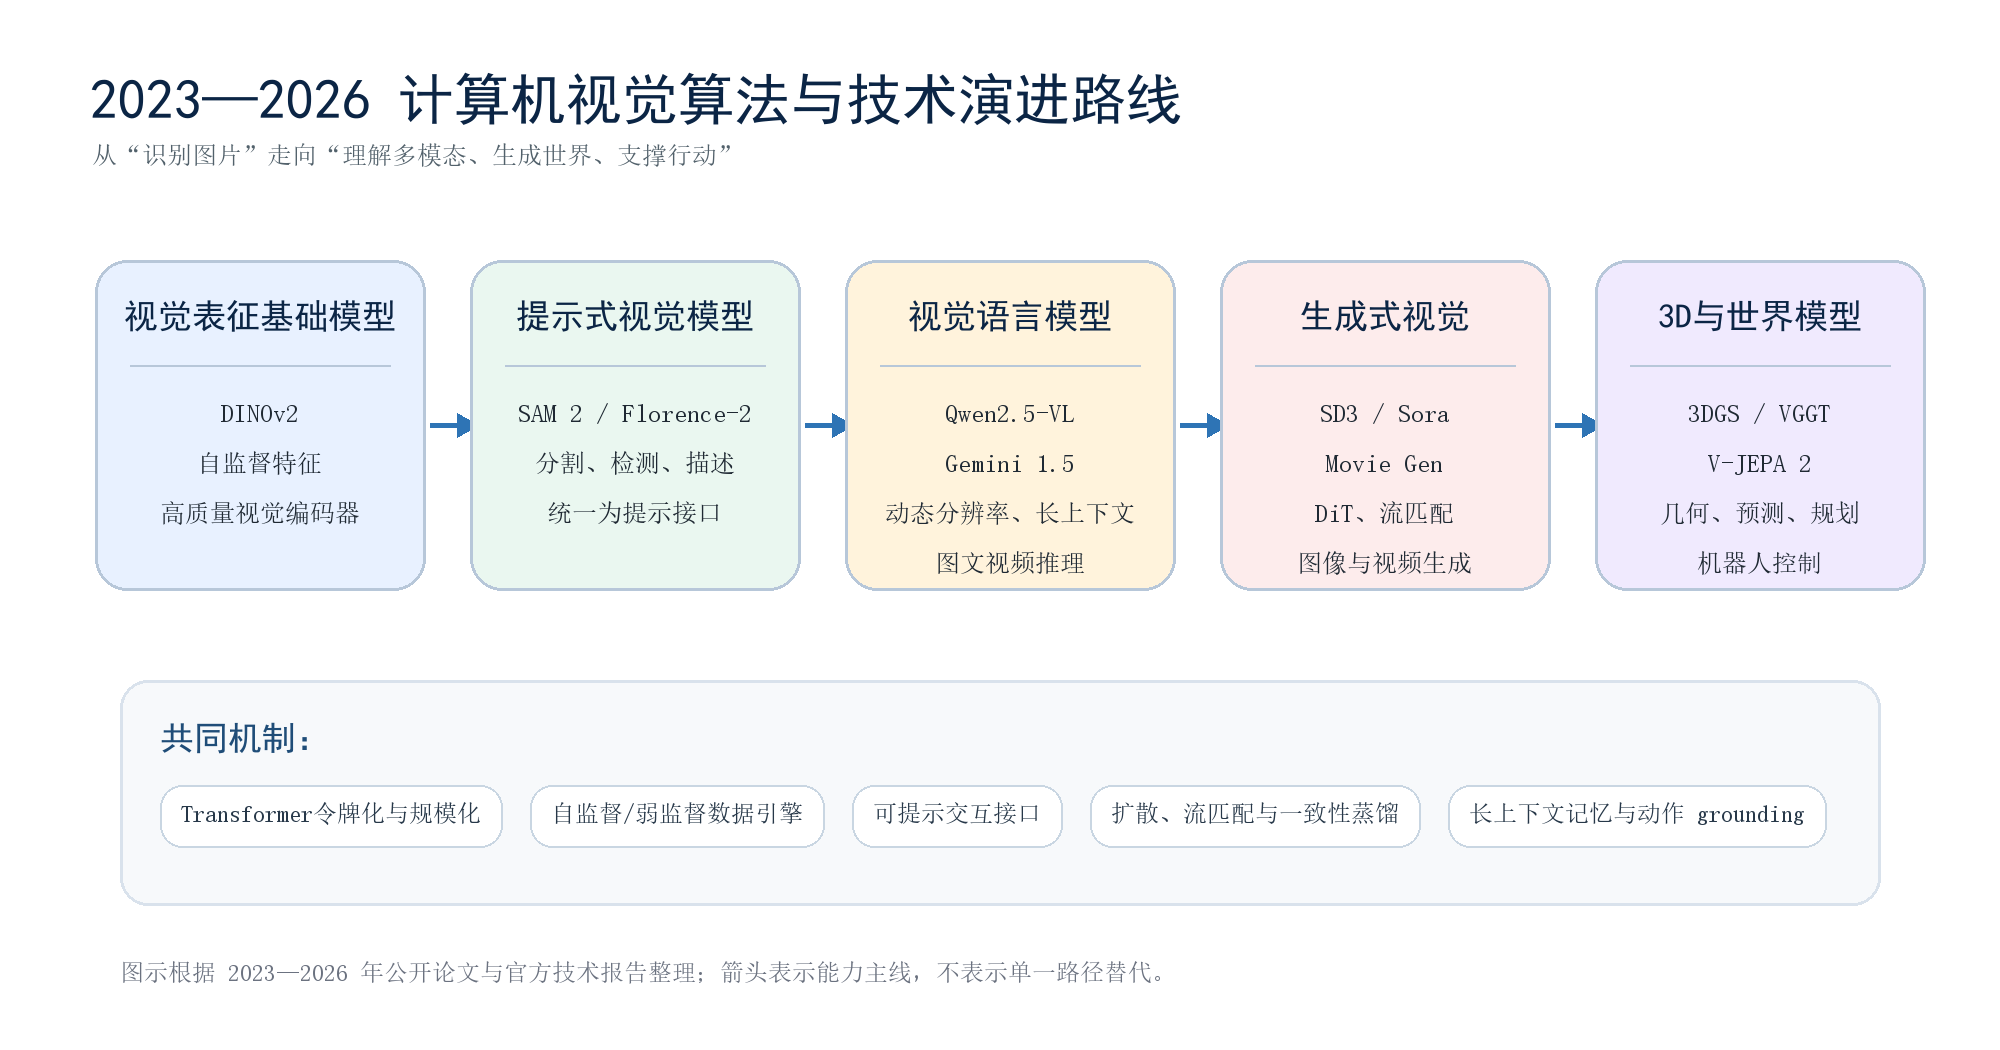
\includegraphics[width=\textwidth]{cv_foundation_model_roadmap.png}
  \caption{2023—2026年计算机视觉算法与技术演进路线}
  \label{fig:roadmap}
\end{figure}

\begin{table}[htbp]
\centering
\small
\caption{计算机视觉最新进展的主线归纳}
\begin{tabularx}{\textwidth}{C{2.2cm}Y Y Y}
\toprule
\textbf{技术主线} & \textbf{代表模型/技术} & \textbf{核心机制} & \textbf{意义} \\
\midrule
通用表征 & \model{DINOv2}、\model{SAM 2}、\model{Florence-2} & 自监督学习、提示式分割、统一任务序列化 & 降低迁移成本，使视觉能力可复用 \\
多模态推理 & \model{Qwen2.5-VL}、\model{Gemini 1.5}、\model{GPT-4o}、\model{LLaVA-OneVision} & 动态分辨率、长上下文、图文视频联合推理 & 视觉系统从识别走向解释、对话和任务执行 \\
开放词汇与密集预测 & \model{YOLO-World}、\model{Depth Anything V2} & 文本条件检测、大规模弱监督/合成数据 & 减少类别封闭假设，提升真实场景适应性 \\
生成式视觉 & \model{SD3}、\model{PIXART-$\delta$}、\model{DyDiT}、\model{Sora}、\model{Movie Gen} & DiT、整流流、一致性蒸馏、时空潜变量 & 提高内容生产、仿真和视频编辑能力 \\
三维与具身智能 & \model{3DGS}、\model{pixelSplat}、\model{VGGT}、\model{OpenVLA}、$\pi_0$、\model{V-JEPA 2} & 显式高斯表示、多视图Transformer、VLA动作头、预测式世界模型 & 连接机器人、AR/VR和物理世界任务 \\
\bottomrule
\end{tabularx}
\end{table}

\section{正文：算法与技术的最新进展}
\subsection{视觉基础模型：从专用网络到通用表征}
早期深度视觉模型通常围绕ImageNet分类、COCO检测或特定分割数据集优化，模型结构与训练目标高度绑定。\model{DINOv2}的意义在于，它把自监督视觉特征训练提升到基础模型层面：模型不依赖人工类别标签，而是通过视觉自身的相似性、局部—全局一致性和大规模数据过滤形成可迁移特征\cite{dinov2}。这种特征对下游任务有两个价值：一是减少标注成本，二是让不同任务共享同一个视觉编码器，便于工业系统中的统一部署。

\model{SAM 2}代表了另一个方向：不是只输出一个固定类别，而是让用户用点、框、掩码或历史记忆提示模型分割目标。相比图像版SAM，\model{SAM 2}面向视频引入streaming memory，使模型能在连续帧中保持目标信息，并通过model-in-the-loop数据引擎不断改善交互质量\cite{sam2}。这类模型适合医疗影像轮廓标注、工业缺陷定位、视频编辑和遥感对象提取等场景。它的启示是，未来视觉模型的交互方式将更接近“协作式标注助手”，而不只是一次性预测器。

\model{Florence-2}进一步提出统一任务接口：把视觉任务都表示为文本提示和序列输出，例如“请描述图像”“请找出某物体位置”“请输出区域掩码”等\cite{florence2}。这与大语言模型的指令范式相似，使视觉系统能够通过自然语言或结构化提示选择任务。从课程知识角度看，这并没有否定传统图像处理和几何视觉，而是把底层特征、区域、边界和语义包装成更高层的可调用能力。

从“专用网络”走向“基础模型”的关键并不只是参数规模增大，而是训练目标、数据组织和接口方式同时发生变化。第一代\model{SAM}的贡献在于把交互式分割抽象为“提示—掩码”问题，构建了大规模SA-1B数据集，使分割模型第一次具有接近工具平台的通用性\cite{sam}。\model{SAM 2}继续沿着这一思路把数据引擎扩展到视频：模型输出不再是孤立图像上的静态区域，而是随时间演化的masklet。这一变化对课程中的图像配准和视频目标跟踪很有启发，因为“同一目标在不同帧中保持身份”本质上就是跨帧对应关系的学习化表达。

自监督表征路线也在继续推进。\model{DINOv3}在\model{DINOv2}基础上强调更长训练、更大数据与稠密特征稳定性，并提出Gram anchoring以缓解长训练中密集特征退化的问题\cite{dinov3}。这说明自监督学习并不是被视觉语言模型替代的旧路线，而是很多多模态系统的视觉底座：如果视觉编码器不能稳定产生局部、边界和几何信息，后续语言模型再强也只能在不可靠的视觉token上推理。\model{SigLIP 2}则从图文对齐编码器角度补强多语言、定位和稠密预测能力\cite{siglip2}，说明未来视觉编码器不仅要做检索和分类，还要支持OCR、区域定位、跨语言语义对齐和多分辨率输入。

这些模型也暴露出基础模型化的三个边界。其一，数据引擎本身会影响模型偏好：如果数据中某些场景、文化符号或工业缺陷样本不足，模型就可能在开放世界中表现不稳定。其二，可提示接口降低了使用门槛，却不等于模型真正理解任务目标；用户给出的点、框和文本提示若含糊，模型可能给出看似合理但不符合业务定义的结果。其三，统一模型容易带来“平均能力强、专业任务不够稳”的问题，例如医学边界、透明材质和细粒度工业缺陷仍需要领域数据微调和人工复核。因此，课程报告不能只把基础模型写成“万能模型”，更应把它理解为可复用视觉能力层。

从工程系统看，视觉基础模型最适合承担三类角色。第一是预标注器，在数据标注前给出候选框、候选掩码或候选区域，缩短人工标注时间。第二是通用特征提取器，为检索、聚类、异常检测和小样本分类提供统一表征。第三是交互式视觉工具，把用户的自然语言、点击、框选和历史修订转化为结构化视觉输出。若与课程中的预处理、标定、配准和误差分析结合，这些模型就能从论文中的demo变成可部署流程：先保证图像质量和几何坐标，再调用模型生成候选结果，最后通过指标与人工反馈闭环改进。

\subsection{视觉语言模型：从看图问答到多模态推理}
视觉语言模型的发展速度尤其快。2024年的\model{Qwen2-VL}强调“任意分辨率”感知，通过动态分辨率把不同尺寸图像转化为不同数量视觉token，并结合多维旋转位置编码处理二维图像和视频时间信息\cite{qwen2vl}。2025年的\model{Qwen2.5-VL}继续加强文档解析、细粒度定位、视频事件理解和视觉agent能力\cite{qwen25vl}。这类设计解决了一个实际痛点：真实图像并不总是固定尺寸，文档截图、医学图像、监控画面和长视频都可能因为缩放而丢失关键信息。

\model{Gemini 1.5}展示了另一种能力路线：超长上下文。论文报告模型能够处理包含长文本、长视频、音频和代码的百万级上下文\cite{gemini15}。对于计算机视觉而言，长上下文意味着模型可以一次性理解更完整的过程，例如一段实验视频的全部步骤、一场课堂录屏的关键节点，或一组多视角图像之间的关系。\model{GPT-4o}和其他原生多模态模型则强调低延迟音视频交互，使视觉理解更接近实时人机协作\cite{gpt4o}。

开源视觉语言模型也在缩小与闭源模型的差距。\model{LLaVA-OneVision}通过统一单图、多图和视频任务迁移，说明视觉语言模型可以从单图对话扩展到跨媒体理解\cite{llavaov}。\model{PaliGemma 2}和\model{Idefics2}等模型表明，紧凑视觉编码器、语言模型和高质量训练流程结合后，也能在OCR、图像描述、细粒度识别和文档理解中取得实用效果\cite{paligemma2,idefics2}。这对教学和科研尤其重要，因为开放模型便于复现实验、理解机制和构建国产化应用。

视觉语言模型的技术难点可以概括为“看得细、记得久、答得准”。“看得细”要求模型在高分辨率图像中保留小目标、文字、表格线和空间关系；如果简单把图像缩放到固定尺寸，车牌、病灶、仪表盘数字或电路板焊点都会被压缩掉。“记得久”要求模型在长视频或多页文档中保持事件链和对象身份，而不是只理解当前帧。“答得准”则要求模型把视觉证据与语言输出绑定起来，避免把语言模型的常识幻觉当成图像事实。动态分辨率、区域裁剪、多尺度token、长上下文和检索增强，都是围绕这三个问题展开的。

从模型结构看，当前视觉语言模型通常由视觉编码器、投影层和语言模型三部分组成。视觉编码器把图像划分为patch或区域特征，投影层把视觉特征映射到语言模型可处理的嵌入空间，语言模型再根据用户指令生成文本、坐标、代码或工具调用。这个结构看似简单，但细节差异很大：有的模型把图像压成少量全局token，适合对话但不利于定位；有的模型保留大量局部token，定位更强但计算成本高；有的模型引入多维位置编码，显式区分图像二维位置和视频时间位置。理解这些差异，有助于解释为什么同样是“看图说话”，不同模型在OCR、图表理解和长视频问答上的表现会相差很大。

视觉语言模型的评价也应比普通图像分类更严格。对课程报告而言，可以把模型输出分成四层：事实层、空间层、推理层和行动层。事实层考察模型是否识别出图像中的对象和文字；空间层考察模型是否能说明“左上角”“前后关系”“遮挡关系”等视觉结构；推理层考察模型能否根据图表、文档和多帧事件作出合理判断；行动层则考察模型是否能把视觉理解转化为工具调用、机器人动作或实验步骤。若模型在事实层已有错误，就不应继续信任其复杂推理。因此，优秀的视觉语言系统应能引用视觉证据、承认不确定性，并在高风险场景中触发人工复核。

\begin{table}[htbp]
\centering
\small
\caption{视觉语言模型能力分层与典型风险}
\begin{tabularx}{\textwidth}{C{2.4cm}Y Y Y}
\toprule
\textbf{能力层} & \textbf{典型任务} & \textbf{关键指标} & \textbf{主要风险} \\
\midrule
事实感知 & 识别物体、文字、颜色和数量 & OCR准确率、对象召回率、描述一致性 & 漏检小目标、误读文字、把背景当主体 \\
空间理解 & 解析位置、遮挡、方向和几何关系 & 定位误差、grounding准确率、区域一致性 & 坐标漂移、左右混淆、遮挡对象误判 \\
跨帧推理 & 长视频问答、事件总结、过程追踪 & 事件召回、时间定位、对象身份保持 & 忘记早期事件、身份漂移、因果倒置 \\
任务行动 & 工具调用、UI操作、机器人指令生成 & 任务成功率、错误恢复率、安全拒答率 & 幻觉操作、越权执行、缺少人工确认 \\
\bottomrule
\end{tabularx}
\end{table}

因此，视觉语言模型的先进性不能只看“回答是否流畅”。在课程学习中，更值得关注的是它如何把视觉特征、位置编码、上下文窗口和语言推理组织成系统能力。一个高水平报告应明确指出：视觉语言模型并没有消除传统视觉误差，而是把误差从像素空间传递到语义空间；一旦模型把模糊图像解释成确定事实，风险反而更隐蔽。把这类模型用于教育、医疗、交通和工业场景时，必须保留原始图像证据、版本信息、提示词和输出日志，便于事后复核。

\subsection{开放词汇检测、分割与几何估计}
真实世界的视觉任务往往存在开放类别。传统检测器需要预先定义类别集合，遇到训练集中没有的对象就会失效。\model{YOLO-World}把文本嵌入与实时检测框架结合，使检测器能够根据文本提示识别开放词汇目标\cite{yoloworld}。这类方法适合仓储盘点、安防巡检、机器人抓取等场景，因为用户可以临时指定要找的对象，而不是重新标注并训练整个检测器。

密集几何估计也出现基础模型化趋势。\model{Depth Anything V2}通过大规模数据和更强教师模型提升单目深度估计泛化能力\cite{depthanythingv2}。单目深度本质上是不适定问题，因为一张图像缺少真实尺度；但大规模预训练能学习常见场景的几何先验，使模型在自动驾驶、室内导航、AR测量和三维重建中提供更稳定的初值。需要注意的是，深度基础模型仍可能在透明物体、反光表面、极端光照和罕见场景中失效，因此工程应用必须结合相机标定、多传感器融合和异常检测。

开放词汇视觉的核心是把“类别集合”从训练阶段移动到推理阶段。传统检测器的类别通常写死在数据集标签中，例如COCO的80类；开放词汇检测器则把文本作为条件输入，让用户在推理时指定“安全帽”“裂纹”“红色阀门”“左侧仪表”等对象。这种变化对工业、安防和机器人很重要，因为真实任务的对象集合经常变化，重新采集标注数据和训练模型成本很高。但是开放词汇能力也带来新的误差：模型可能把语义相近的类别混淆，例如“安全帽”和“普通帽子”；也可能因为文本提示过宽，把背景中相似纹理误检为目标。因此开放词汇检测更适合做候选发现，而不适合在无复核情况下直接做最终判定。

分割模型与检测模型的关系也在变化。过去检测输出框、分割输出像素级区域，二者常由不同模型处理；现在提示式分割让框、点、文本和历史掩码都能成为交互入口。对工业缺陷而言，检测框只能告诉我们缺陷大概在哪里，掩码才能支持面积、周长、裂纹长度和缺陷比例等测量。对医学影像而言，掩码边界直接影响体积估计和手术规划。也就是说，开放词汇检测回答“找什么”，提示式分割回答“边界在哪里”，几何估计回答“离相机多远、在空间何处”。三者结合后，视觉系统才更接近真实应用需求。

深度估计和几何基础模型需要特别强调尺度问题。单目模型可以产生视觉上合理的相对深度，但机器人抓取、AR测量和车辆避障需要可解释的真实尺度。若没有相机内参、畸变校正和场景约束，深度图可能在局部看起来平滑，却在真实三维坐标中产生明显误差。因此，将\model{Depth Anything V2}等模型用于工程时，常见做法不是完全替代几何，而是用学习模型提供稠密初值，再用双目、激光雷达、结构光、PnP或bundle adjustment进行尺度校正。这个思路体现了现代视觉的融合趋势：数据驱动提供先验，几何模型提供硬约束。

\begin{table}[htbp]
\centering
\small
\caption{开放词汇检测、提示式分割与几何估计的互补关系}
\begin{tabularx}{\textwidth}{C{2.4cm}Y Y Y}
\toprule
\textbf{任务} & \textbf{输入形式} & \textbf{输出结果} & \textbf{适合解决的问题} \\
\midrule
开放词汇检测 & 文本提示、图像、少量候选框 & 目标类别与边界框 & 新类别目标发现、快速巡检、候选区域筛选 \\
提示式分割 & 点、框、掩码、文本或视频记忆 & 像素级目标区域 & 精细轮廓标注、面积测量、视频对象跟踪 \\
单目深度估计 & 单张图像或视频帧 & 相对/伪尺度深度图 & 三维初值、导航提示、场景结构理解 \\
几何校正 & 相机内外参、多视图对应、传感器数据 & 真实尺度位姿、点云或重建模型 & 机器人操作、AR叠加、可验证三维测量 \\
\bottomrule
\end{tabularx}
\end{table}

从课程角度看，这一部分最能体现“新旧知识连接”。边缘检测和特征匹配仍然解释了为什么模型需要局部结构；相机标定解释了为什么深度估计需要尺度约束；图像配准解释了为什么视频分割需要保持目标身份。最新模型把这些问题放进神经网络中学习，但问题本身没有消失。对学生而言，真正的能力不是记住某个模型名称，而是能够判断在具体场景中应使用检测、分割、深度、配准还是多传感器融合，并能说清楚每一步的误差来源。

\subsection{生成式图像与视频：从合成内容到世界模拟}
生成式视觉的核心变化是骨干结构和采样方式的变化。\model{Stable Diffusion 3}使用多模态扩散Transformer与整流流训练，说明扩散模型正在从U-Net主干走向Transformer主干，并更重视文本—图像对齐和高分辨率生成\cite{sd3}。\model{PIXART-$\delta$}通过潜空间一致性模型把高质量图像生成压缩到少步采样\cite{pixartdelta}，\model{DyDiT}则尝试根据时间步和空间token动态调整扩散Transformer计算量\cite{dydit}。这些工作说明生成模型的竞争不再只是“画得更逼真”，还包括更快、更可控、更低成本。

视频生成是近年最受关注的方向。\model{Sora}官方技术报告将视频和图像表示为时空patch，并在压缩后的潜空间中训练生成模型，使同一框架能够处理不同长度、分辨率和宽高比的视频\cite{sora}。\model{Movie Gen}进一步覆盖文本生成视频、个性化视频、视频编辑和音频生成，被定位为一组媒体基础模型\cite{moviegen}。\model{Veo}系列则展示了高质量视频生成、镜头控制和声音结合能力\cite{veo}。这些模型让视觉生成从静态图片合成走向内容生产流程，但也带来深度伪造、版权归属、训练数据透明度和物理一致性不足等问题。

把视频生成称为“世界模拟器”并不意味着模型真正理解物理定律。更准确地说，模型学到了大量视觉动态的统计规律：物体如何移动，镜头如何变化，动作如何影响场景。当这些规律足够强时，模型可以为机器人训练、自动驾驶仿真和影视预演提供低成本数据。但它仍可能在因果关系、物体守恒、长期一致性和可控性方面出错，所以不能把生成视频直接等同于可靠仿真。

视频扩散模型的发展可以从两个层面理解。第一层是生成质量：模型需要在每一帧中保持清晰度、纹理细节和主体一致性。第二层是时间建模：模型需要在多个帧之间保持动作连续、场景布局稳定和物体身份不漂移。\model{Stable Video Diffusion}强调从图像模型扩展到视频模型时，数据策划和运动表示同样关键\cite{svd}；\model{Lumiere}提出space-time U-Net，一次性生成完整时间段，而不是只用逐段拼接方式生成视频\cite{lumiere}。这些方法都在尝试减少视频生成中的闪烁、跳帧和局部不一致问题。

进入2025年以后，视频生成系统开始更重视可控性与安全发布。\model{Sora 2}系统卡强调视频与音频生成能力，也讨论了同步音频、真实人物相似性、错误信息和安全缓解措施\cite{sora2}。\model{Veo 3.1}等官方模型进一步展示了镜头控制、声音生成和编辑能力\cite{veo}。这说明生成式视觉已经不再只是“给一句提示生成一段短视频”，而是在向完整媒体生产系统演化：用户希望控制镜头、角色、动作、声音、风格和后期修改。对课程报告而言，这一趋势值得关注，因为它把传统视觉中的运动估计、视频分割、三维几何和多模态理解都重新纳入生成流程。

生成式视觉也改变了数据增强的含义。传统数据增强通常是旋转、裁剪、加噪声或颜色扰动，本质上是在已有样本附近制造局部变化；生成式模型则可以合成罕见天气、罕见缺陷、危险交通场景或不同相机视角。若使用得当，它能帮助训练集覆盖长尾情形，降低真实采集成本。但生成数据必须被严格标注来源，并与真实数据分开评估。原因很简单：生成模型可能复制训练数据偏见，也可能产生现实中不可能出现的几何结构。如果把这类数据直接混入训练集而不做质量控制，模型可能学到错误先验。

因此，生成式视觉的评价应至少包含四个维度。第一是感知质量，即画面是否清晰、细节是否自然；第二是语义一致性，即生成内容是否符合文本或图像条件；第三是时空一致性，即物体、身份和场景布局是否随时间稳定；第四是任务可用性，即生成结果能否帮助下游检测、分割、三维重建或机器人训练。许多视频看起来很震撼，但如果不能保持交通信号灯状态、车辆轨迹和碰撞逻辑，就不能作为自动驾驶仿真数据。高水平的视觉报告应把“好看”和“可验证”区分开来。

\begin{table}[htbp]
\centering
\small
\caption{生成式视觉从图像到世界模拟的能力层级}
\begin{tabularx}{\textwidth}{C{2.6cm}Y Y Y}
\toprule
\textbf{层级} & \textbf{代表技术} & \textbf{主要能力} & \textbf{尚未解决的问题} \\
\midrule
图像生成 & 扩散模型、DiT、整流流 & 高分辨率图像合成、风格控制、局部编辑 & 精确文字、复杂空间关系、版权边界 \\
短视频生成 & 视频扩散、时空潜变量 & 动作连续、镜头运动、短时一致性 & 长期身份保持、物体守恒、复杂交互 \\
媒体基础模型 & Movie Gen、Veo、Sora 2 & 视频、音频、编辑、个性化角色 & 可控性、安全发布、真实人物保护 \\
交互世界模型 & Genie、Genie 3、V-JEPA路线 & 可操作环境、预测、规划和仿真 & 物理真实性、长时任务、可验证评估 \\
\bottomrule
\end{tabularx}
\end{table}

\subsection{三维重建、多视图视觉与可编辑资产}
三维视觉长期依赖多视图几何、SLAM、NeRF和深度传感器。2023年的\model{3D Gaussian Splatting}用显式三维高斯表示场景，在保证较高渲染质量的同时实现实时新视角渲染\cite{gs3d}。与需要大量体渲染采样的NeRF相比，高斯表示更适合交互式浏览、编辑和AR/VR显示。\model{pixelSplat}则从图像对直接预测3D Gaussian，使可泛化三维重建更接近即时生成\cite{pixelsplat}。

2025年的\model{VGGT}把视觉几何任务进一步统一化：模型尝试从一个或多个视图中预测相机参数、深度图、点云和跟踪信息\cite{vggt}。这与课程中相机标定、图像配准和三维重建的知识直接相关。传统方法强调几何约束和优化，基础模型强调数据驱动的先验与端到端预测。更合理的未来方向不是二选一，而是把深度学习的强先验与几何约束结合起来：用模型给出初值和语义理解，用几何优化保证尺度、位姿和一致性。

要理解三维视觉近年的变化，需要先区分三件事：表示、渲染和定位。NeRF类方法把场景表示为连续辐射场，优势是新视角合成质量高，但训练和渲染成本较高。\model{Zip-NeRF}通过抗锯齿和grid-based表示改进多尺度渲染质量\cite{zipnerf}，说明NeRF路线仍在追求质量、速度和尺度一致性的平衡。\model{3D Gaussian Splatting}则采用显式高斯点云，每个高斯携带位置、尺度、方向、不透明度和颜色等参数，渲染时通过splatting快速投影到图像平面，因此更容易实现实时交互\cite{gs3d}。这也是它迅速受到AR/VR、数字孪生和游戏资产领域关注的重要原因。

但是，高质量渲染并不等于完整场景理解。3DGS可以很好地重建外观，却未必知道哪个高斯属于桌子、墙面或行人；它能渲染新视角，却不一定能回答场景中物体的功能关系。为了从“可看”走向“可用”，研究者开始把高斯表示与SLAM、语义分割和动态场景建模结合。例如\model{GS-SLAM}尝试把3D Gaussian用于稠密视觉SLAM，在相机定位和地图构建之间共享显式三维表示\cite{gsslam}。这类工作说明三维视觉正在从离线重建走向在线定位、实时更新和机器人导航。

多视图几何基础模型提供了另一条路线。传统SfM和MVS依赖特征匹配、三角化、bundle adjustment等步骤，优点是几何含义清晰，缺点是在弱纹理、反光、重复结构和大视角差下容易失败。以\model{VGGT}为代表的模型尝试用Transformer一次性预测相机、深度和点云，把长期积累的几何流程压缩进学习系统。它的优势是速度快、对稀疏输入友好；局限是需要大量多视图训练数据，且在高精度测量时仍需几何校验。对课程学习而言，这正好说明“标定、配准和三维重建”不是过时章节，而是理解前沿模型可靠性的基准。

\begin{table}[htbp]
\centering
\small
\caption{三维视觉表示路线对比}
\begin{tabularx}{\textwidth}{C{2.4cm}Y Y Y}
\toprule
\textbf{路线} & \textbf{核心思想} & \textbf{优势} & \textbf{局限} \\
\midrule
多视图几何 & 特征匹配、三角化、bundle adjustment & 可解释、尺度和误差可分析 & 弱纹理和大视角差下易失败，流程较复杂 \\
NeRF/Zip-NeRF & 用神经辐射场表示连续场景 & 视角合成质量高，适合静态场景重建 & 训练/渲染成本较高，交互编辑不够直接 \\
3DGS & 显式三维高斯点云实时投影渲染 & 实时新视角、可编辑、适合交互展示 & 语义理解弱，动态场景和物理约束仍难 \\
几何Transformer & 端到端预测相机、深度、点云和跟踪 & 统一任务接口、速度快、适合泛化初值 & 精度和尺度仍需几何优化或传感器校正 \\
\bottomrule
\end{tabularx}
\end{table}

三维视觉的应用价值在于它把视觉从二维图像推向空间操作。工业检测中，二维图像可以发现表面缺陷，但三维模型才能测量装配间隙和形变；文化遗产保护中，照片可以记录纹理，但三维重建才能支持远程展览和数字修复；机器人操作中，识别物体类别只是第一步，抓取还需要位姿、尺度和可达性。未来高水平系统很可能采用组合式架构：视觉基础模型负责语义和区域，三维表示负责空间和外观，几何优化负责一致性，机器人或AR系统负责交互执行。

\subsection{世界模型与具身智能：从理解到行动}
计算机视觉的最终目标之一是让机器理解并参与真实世界。\model{OpenVLA}把视觉语言模型接入机器人动作输出，形成开源视觉—语言—动作模型\cite{openvla}；$\pi_0$使用视觉语言条件和flow matching策略学习通用机器人控制\cite{pi0}。这些方法把视觉输入、语言指令和低层动作连接起来，使模型不只回答“图中有什么”，还要决定“接下来怎么做”。

\model{V-JEPA 2}代表预测式世界模型路线：模型通过自监督视频学习形成对未来状态和场景变化的预测能力，并把理解、预测和规划连接起来\cite{vjepa2}。\model{Genie 2}则把世界模型用于可交互环境生成，强调从图像或文本提示中生成可操作的虚拟世界\cite{genie2}。这说明视觉算法正在进入一个新的问题域：模型需要理解时间、因果、动作结果和任务目标。从算法角度看，这要求更好的长时记忆、物理一致性、可验证规划和跨机器人平台泛化。

具身智能可以理解为视觉、语言和动作的闭环。传统视觉系统通常以“识别正确”为目标，而机器人系统必须进一步考虑“动作是否安全、是否达成目标、失败后能否恢复”。\model{RT-2}把机器人动作离散化为类似文本token的形式，使模型能够把网络图文知识迁移到真实机器人控制中\cite{rt2}。\model{OpenVLA}则强调开放模型和真实机器人示教数据，使研究者能够在较低成本下微调和复现VLA能力\cite{openvla}。这些工作共同说明，视觉语言模型正在从回答问题的助手，变成能够生成动作方案的控制接口。

世界模型路线并不完全等同于VLA。VLA关注从当前观察和指令到动作的映射，世界模型更关注“如果采取某个动作，未来会发生什么”。\model{DreamerV3}代表模型化强化学习路线：智能体先学习环境动态模型，再在想象空间中进行策略学习\cite{dreamerv3}。\model{Genie}和\model{Genie 3}代表生成式可交互环境路线：模型从图像、文本或视频中生成可操作世界，为智能体提供低成本试错空间\cite{genie,genie3}。\model{V-JEPA 2}则代表表征预测路线：模型不直接重建每个像素，而是在抽象表征空间中预测未来，以支持理解、预测和规划\cite{vjepa2}。这三条路线分别对应控制、仿真和表征，它们未来可能融合。

世界模型之所以重要，是因为现实世界中的数据采集成本极高。机器人若每次学习都必须在真实环境中试错，既慢又危险；自动驾驶若只依赖真实道路收集极端事故样本，也不现实。世界模型提供了一种可能：先在学习到的环境中想象不同动作后果，再把少量最有价值的策略带到真实世界验证。但这也带来新的风险。如果世界模型对物理规律、接触力、摩擦、遮挡或人类行为预测不准，智能体可能在虚拟环境中学会现实中不可行甚至危险的策略。

因此，世界模型的关键评价不是“生成画面是否逼真”，而是“预测是否可用于决策”。一个模型可以生成很真实的视频，却不能准确预测杯子被推倒后的轨迹；也可以生成可交互场景，却在长时间操作中逐渐偏离物理逻辑。对于VLA和世界模型，评价应包括任务成功率、长时一致性、异常恢复、安全约束遵守、跨场景泛化和人类接管频率。课程中的误差分析思想在这里同样适用：只不过误差不再只是像素误差或重投影误差，而是动作后果误差和安全风险。

\begin{table}[htbp]
\centering
\small
\caption{从视觉理解到世界模型的三条路线}
\begin{tabularx}{\textwidth}{C{2.5cm}Y Y Y}
\toprule
\textbf{路线} & \textbf{代表工作} & \textbf{核心问题} & \textbf{评价重点} \\
\midrule
视觉语言动作模型 & RT-2、OpenVLA、$\pi_0$ & 如何把视觉观察和语言指令转化为机器人动作 & 任务成功率、动作安全、跨机器人泛化 \\
模型化强化学习 & DreamerV3等 & 如何学习环境动态并在想象空间中优化策略 & 样本效率、长期回报、真实迁移能力 \\
生成式世界模型 & Genie、Genie 3、Sora路线 & 如何生成可交互、可控制、可预测的环境 & 交互一致性、物理真实性、可验证仿真 \\
表征预测模型 & V-JEPA 2等 & 如何在抽象表征空间中预测未来状态 & 预测稳定性、规划能力、少量真实数据适配 \\
\bottomrule
\end{tabularx}
\end{table}

\begin{table}[htbp]
\centering
\small
\caption{代表性最新视觉算法与技术对照}
\begin{tabularx}{\textwidth}{C{2.45cm}C{1.75cm}C{2.05cm}Y Y}
\toprule
\textbf{模型/技术} & \textbf{年份} & \textbf{类型} & \textbf{核心机制} & \textbf{典型应用} \\
\midrule
\model{DINOv2} & 2023 & 自监督视觉表征 & 无标注特征学习、数据过滤、大规模ViT & 迁移分类、检索、密集预测 \\
\model{SAM 2} & 2024 & 提示式图像/视频分割 & 流式记忆、交互提示、数据引擎 & 视频目标分割、医学/工业标注 \\
\model{Qwen2.5-VL} & 2025 & 视觉语言模型 & 动态分辨率、定位、长视频和文档理解 & 多模态助手、OCR、视觉agent \\
\model{Sora}/\model{Movie Gen} & 2024 & 视频生成 & 时空潜变量、DiT/扩散、音视频生成与编辑 & 内容创作、仿真、视频后期 \\
\model{3DGS}/\model{VGGT} & 2023/2025 & 三维视觉 & 显式高斯表示、多视图几何Transformer & AR/VR、数字孪生、机器人感知 \\
\model{OpenVLA}/$\pi_0$ & 2024 & 具身智能 & VLM接动作头、flow policy、机器人演示数据 & 机器人控制、通用操作任务 \\
\bottomrule
\end{tabularx}
\end{table}

\section{从课程基础到前沿模型的知识连接}
本课程前半部分讲到的图像处理基础、相机模型、相机标定和图像配准，并不是被大模型时代淘汰的旧知识。相反，越是复杂的视觉基础模型，越需要这些基础概念来解释其输入、约束和失效边界。许多新模型在论文中看起来是端到端系统，但工程落地时仍要回答三个传统问题：图像信号是否可靠，视角和尺度是否可解释，多帧或多视图之间是否一致。没有这些基础，模型输出就容易停留在“看起来合理”，而不能成为可验证、可部署的视觉系统。

首先，图像处理基础仍然决定模型输入质量。传统课程中的去噪、增强、直方图均衡、边缘和纹理分析，本质上是在改善像素分布和局部结构，使后续算法更容易提取稳定特征。深度视觉模型虽然把滤波器、边缘和纹理特征交给网络自动学习，但它们仍然受到噪声、模糊、曝光不足、运动拖影和压缩伪影影响。例如工业相机拍摄高速流水线时，若光照不稳定或快门设置不当，\model{SAM 2}的分割边界、\model{YOLO-World}的检测框和视觉语言模型的文本解释都可能同时退化。因此，现代视觉系统并不是“直接把图片丢给大模型”，而是需要在采集、预处理、模型推理和后处理之间建立完整链路。

其次，相机模型和相机标定仍是三维视觉的坐标基础。课程中的针孔相机模型、内参、外参、畸变校正和重投影误差，回答的是二维图像如何对应三维空间的问题。\model{VGGT}、\model{Depth Anything V2}、\model{3D Gaussian Splatting}等前沿模型能够从数据中学习几何先验，但如果要进行真实尺度测量、机器人抓取或AR叠加，仍必须知道相机坐标系与世界坐标系之间的关系。单目深度模型可以给出相对深度趋势，却未必给出可直接用于机械臂控制的米制尺度；高斯重建可以生成逼真视角，却可能在尺度漂移或相机位姿不准时产生局部扭曲。由此可见，几何视觉的价值从“手工设计完整算法”转向“为学习模型提供约束和校验”。

再次，图像配准和特征匹配是视频理解、三维重建和世界模型的隐含基础。传统配准关注关键点、描述子、单应矩阵、基础矩阵和光流估计，目标是让不同图像或不同帧中的同一结构对齐。视频基础模型虽然使用Transformer token、时序位置编码或记忆模块，但它们仍要解决同一个问题：跨帧目标如何保持身份，遮挡后如何恢复，摄像机运动和物体运动如何区分。\model{SAM 2}的streaming memory可以看作一种学习到的跨帧配准和目标记忆；视频生成模型中的时空patch建模，也是在高维潜空间中维持帧间一致性。若模型无法保持配准一致，生成视频就会出现物体形变、纹理跳变或身份漂移。

最后，误差分析和鲁棒性评估是传统视觉与基础模型共同面对的问题。相机标定中有重投影误差，图像配准中有匹配误差，深度估计中有尺度误差，视觉语言模型中则有语义幻觉和定位错误。不同任务的误差形式不同，但都需要被量化和追踪。一个可靠系统不应只输出答案，还应输出置信度、失败提示和可复核证据。例如在医疗图像分割中，模型给出病灶区域后应保留原图、提示点、版本号和人工修订记录；在自动驾驶仿真中，世界模型生成的视频不能只看视觉质量，还要评估交通规则、物体轨迹和碰撞逻辑是否一致。

\begin{table}[htbp]
\centering
\small
\caption{课程基础知识与最新视觉模型的对应关系}
\begin{tabularx}{\textwidth}{C{2.5cm}Y Y Y}
\toprule
\textbf{课程知识点} & \textbf{核心问题} & \textbf{前沿模型中的体现} & \textbf{工程启示} \\
\midrule
图像处理基础 & 如何获得清晰、稳定、可分析的像素输入 & 视觉编码器对噪声、模糊和曝光变化仍敏感 & 采集与预处理质量会直接影响模型上限 \\
相机模型与标定 & 二维图像如何对应三维空间坐标 & \model{VGGT}、\model{Depth Anything V2}需要几何尺度校验 & 学习模型适合给初值，真实测量仍要几何约束 \\
图像配准 & 多视角、多帧之间如何保持对应关系 & \model{SAM 2}记忆模块和视频模型时空token都需保持一致性 & 视频理解和生成要同时关注语义与时序稳定 \\
三维重建 & 如何从图像恢复可交互空间表示 & \model{3DGS}、\model{pixelSplat}把场景表示推向实时渲染 & 显式三维表示更利于编辑、导航和机器人应用 \\
误差分析 & 预测结果是否可信、何时失效 & VLM幻觉、深度尺度漂移、生成视频物理错误 & 必须建立置信度、人工复核和持续监测机制 \\
\bottomrule
\end{tabularx}
\end{table}

\subsection{图像处理基础：从像素增强到模型输入治理}
图像处理基础在大模型时代仍然重要，原因在于模型输入并不是抽象数据，而是由真实相机、光照、镜头、压缩和传输过程共同决定的像素信号。一个视觉基础模型在公开数据集上表现很好，并不意味着它能自动适应实验室摄像头、手机截图、夜间监控或医学设备。低照度会降低纹理对比度，运动模糊会破坏边缘，JPEG压缩会引入块效应，镜头污渍会产生局部遮挡。这些问题在网络内部不会神奇消失，而是会影响后续token和特征。

传统的滤波、锐化、直方图均衡、色彩校正和边缘检测，本质上是在控制输入分布。现代系统可以把这些步骤做得更自动，例如用学习型去噪、超分辨率和图像增强模型改善输入质量；也可以保留简单而可解释的预处理作为质量门控。例如工业质检系统可以先检测曝光是否过低、图像是否失焦、目标是否超出视野，再决定是否调用大模型。这比直接让视觉语言模型解释所有图像更可靠，因为质量问题应在输入端被发现，而不是在输出端用语言掩盖。

从报告写作角度看，图像处理基础可以帮助我们解释基础模型的失效案例。若\model{SAM 2}在低对比度边界处出现漏分割，问题可能不是分割算法本身，而是成像条件导致边界信息不足。若视觉语言模型误读仪表数字，可能与分辨率、压缩和字体大小有关。把这些问题写清楚，报告就从“模型介绍”上升为“视觉系统分析”。

\subsection{相机模型与标定：前沿模型的尺度锚点}
相机标定是连接二维像素与三维空间的桥梁。针孔相机模型、内参矩阵、外参矩阵、畸变参数和重投影误差，看似是传统几何视觉内容，却是三维基础模型落地时不可绕开的尺度锚点。单目深度模型可以学习相对远近，3DGS可以重建视觉上自然的场景，VGGT可以端到端预测相机和点云；但只要系统要进行测量、抓取、避障或AR叠加，就必须回答“这个像素对应真实世界多远、多大、在哪个坐标系”。

例如机器人抓取一个零件时，视觉语言模型可以识别“蓝色把手”，提示式分割可以给出把手区域，单目深度可以估计相对深度，但机械臂最终需要的是抓取点在机器人坐标系下的位置和姿态。这个坐标转换依赖相机外参和手眼标定。如果忽略标定，模型输出再自然，也无法保证动作安全。类似地，在AR应用中，虚拟物体必须与真实平面稳定对齐；如果相机畸变没有校正，虚拟物体就会出现漂移和错位。

高水平视觉系统往往采用“学习模型 + 几何校验”的组合：先由模型产生候选深度、关键点、分割或相机位姿，再用重投影误差、PnP、RANSAC和bundle adjustment进行筛选与优化。这种组合体现了课程知识的价值：学习模型提供强先验，几何方法提供可解释约束。对学生而言，掌握标定不是为了复古，而是为了知道什么时候不能盲信端到端模型。

\subsection{图像配准：跨帧记忆和多视图理解的底层问题}
图像配准研究的是不同图像之间的对应关系。课程中常见方法包括特征点检测、描述子匹配、RANSAC估计单应矩阵或基础矩阵，以及通过变换把图像对齐。今天的视频分割、长视频理解、三维重建和世界模型仍在处理同一个核心问题：同一个目标在不同帧、不同视角、不同遮挡状态下如何保持一致。

\model{SAM 2}的流式记忆模块可以看作学习化的跨帧对应机制。它不再显式输出SIFT或ORB匹配点，但要完成的任务仍是把上一帧目标信息传播到当前帧。\model{Movie Gen}、\model{Sora 2}等视频生成模型也必须解决时序一致性问题：如果潜空间中的对应关系不稳定，同一人物的衣服、脸部和位置就会在相邻帧中跳变。三维重建中的多视图对应更直接：若匹配错误，相机位姿和点云都会被污染。因此，配准思想是从传统算法到世界模型的隐形主线。

配准还提供了一种可复现实验入口。即使没有昂贵GPU和大模型，也可以用合成图像、已知单应矩阵和噪声扰动验证RANSAC如何剔除错误匹配、估计几何变换并计算重投影误差。本文后续实验小节正是利用这一思路，把课程基础中的配准方法转化为可运行代码，并用指标说明鲁棒性评价的重要性。

\subsection{误差分析：从重投影误差到语义幻觉}
传统视觉中的误差通常可以较清晰地定义：相机标定有重投影误差，配准有匹配误差，深度估计有尺度误差，分割有IoU或Dice。基础模型时代的误差更复杂，因为输出可能是文字、掩码、视频、三维场景或动作。视觉语言模型可能把不存在的物体说成存在，生成视频可能在几秒后破坏物体守恒，VLA模型可能给出看似合理但不可执行的动作。这些错误不一定能用一个标量完全描述。

因此，现代视觉系统需要分层误差分析。输入层要检查图像质量、分辨率、曝光和遮挡；几何层要检查尺度、位姿和跨帧一致性；语义层要检查对象、关系和文本事实；任务层要检查最终动作或决策是否安全。这样的分层框架能把课程中的误差概念扩展到前沿模型。如果报告能够把“重投影误差”和“语义幻觉”放在同一套可信视觉系统中讨论，就会比单纯罗列模型更有深度。

\subsection{课程知识到前沿研究的映射}
综合来看，课程中的图像处理、相机模型、标定、配准和三维重建可以分别对应现代视觉系统的输入治理、空间坐标、几何约束、时序一致性和可交互表示。前沿模型并没有取代这些知识，而是把它们嵌入更大的学习框架中。未来学生如果只会调用模型接口，容易在异常场景中束手无策；如果只会传统算法，又难以利用基础模型的迁移能力。真正的竞争力在于把二者连接起来：用传统视觉理解问题边界，用基础模型提高能力上限，用评价体系确保结果可信。

\section{应用价值与现实挑战}
从应用角度看，最新视觉算法的价值主要体现在四类场景。第一是工业制造。开放词汇检测、视频分割和三维重建可以用于缺陷检测、工件定位、产线安全和数字孪生。第二是医疗与公共服务。提示式分割和多模态文档理解可辅助医生标注病灶、整理影像报告，但必须由专业人员复核，不能替代诊断责任。第三是交通与城市治理。深度估计、视频理解和世界模型可服务自动驾驶仿真、道路风险识别和应急响应。第四是教育、文化和科研。生成式视觉和三维重建可以用于虚拟实验、文物数字化、课程可视化和科研数据增强。

在智能制造场景中，视觉基础模型可以改变传统质检流程。过去一条产线往往需要为每类缺陷分别采集样本、标注数据、训练检测器，遇到新产品或新缺陷时还要重新开发。开放词汇检测和提示式分割使系统能够先用文本或少量交互指定目标，再由模型给出候选区域，最后结合规则、测量和人工复核完成判定。若进一步加入三维重建，系统还能判断零件姿态、装配间隙和表面形变。这样的流程更适合小批量、多品种生产，但它对相机标定、光照稳定、缺陷样本管理和误报控制提出了更高要求。

在医疗与公共服务场景中，计算机视觉的价值不在于替代医生，而在于提高信息处理效率。以医学影像为例，\model{SAM 2}一类模型可以辅助轮廓勾画，视觉语言模型可以帮助整理影像描述和检查记录，三维重建可以辅助术前规划。但医学场景高度敏感，模型必须满足可追溯、可复核和隐私保护要求。尤其是视觉语言模型生成文本时，若把不确定区域描述成确定病灶，或者遗漏关键异常，就会带来严重风险。因此，医疗视觉系统更适合作为“第二读片者”或“标注加速器”，而不是独立决策者。

在交通和城市治理场景中，长视频理解、深度估计和世界模型具有现实意义。城市摄像头、车载摄像头和无人机视频通常包含长时间、多目标、多视角信息，仅靠单帧检测难以判断风险演化。视觉语言模型可以把长视频转化为事件描述，深度模型可以估计道路空间结构，世界模型可以生成罕见危险场景用于仿真训练。但交通系统必须强调实时性和安全冗余：模型推理延迟、夜间雨雾天气、遮挡和镜头污染都可能影响结果。真正可用的系统通常需要视觉模型、雷达、地图、规则引擎和人工调度协同工作。

在教育、文化和科研场景中，生成式视觉与三维视觉能够降低知识可视化门槛。教师可以用生成式图像和视频解释抽象概念，用三维重建展示文物、建筑或实验装置；科研人员可以用合成数据补充罕见样本，用视频模型进行实验方案预演。但这些应用同样需要边界：生成内容必须标注来源，不能把生成图像当作真实实验结果；文化遗产数字化要尊重版权和文物保护规范；教育材料要避免把模型生成的错误细节包装成权威知识。

\begin{table}[htbp]
\centering
\small
\caption{典型应用场景、可用技术与落地约束}
\begin{tabularx}{\textwidth}{C{2.3cm}Y Y Y}
\toprule
\textbf{场景} & \textbf{可用技术} & \textbf{主要收益} & \textbf{关键约束} \\
\midrule
智能制造 & 开放词汇检测、提示式分割、三维重建 & 缩短新缺陷适配周期，提升质检自动化 & 光照、标定、误报率、产线实时性 \\
医疗影像 & 视频/图像分割、VLM报告辅助、三维可视化 & 加速标注和报告整理，辅助术前分析 & 隐私保护、医生复核、责任归属 \\
交通治理 & 长视频理解、深度估计、世界模型仿真 & 识别风险事件，生成罕见场景数据 & 低延迟、多传感器冗余、极端天气鲁棒性 \\
教育科研 & 生成式图像视频、3DGS、可交互可视化 & 降低可视化和实验演示成本 & 内容真实性标注、版权和学术诚信 \\
文化遗产 & 多视图重建、三维资产生成、图像修复 & 支持数字保护、展示和远程传播 & 采集规范、历史真实性、数据长期保存 \\
\bottomrule
\end{tabularx}
\end{table}

挑战同样突出。首先是数据与隐私问题。视觉模型训练常依赖海量图像和视频，若数据来源、授权和脱敏流程不清晰，容易侵犯个人信息和知识产权。其次是可靠性问题。视觉语言模型可能产生幻觉，生成式视频可能违反物理规律，深度估计和三维重建可能在特殊材质或极端场景中失败。再次是算力与能耗问题。基础模型规模越大，对训练算力、推理成本和部署设备的要求越高。最后是评价体系问题。很多榜单只衡量静态数据集表现，却难以评估模型在真实开放环境中的安全性、稳定性和可解释性。

因此，未来视觉系统的工程落地应采用“模型能力 + 任务约束 + 人工复核 + 持续评估”的方式。例如在工业质检中，模型可先给出缺陷候选区域，再由规则或人工复核关键样本；在医疗场景中，模型输出应作为辅助信息并保留审计记录；在生成式内容场景中，应加入水印、来源标注和滥用检测。这样的系统设计比单纯追求模型排行榜更符合现实需求。

\subsection{智能制造案例：从缺陷发现到闭环质检}
智能制造是计算机视觉最容易形成闭环价值的场景之一。一个典型缺陷检测流程可以分为五步：第一，固定相机、光源和拍摄距离，保证输入图像稳定；第二，用开放词汇检测或异常检测模型筛选疑似缺陷区域；第三，用提示式分割获得精细掩码，计算缺陷面积、长度、位置和与零件边缘的关系；第四，用规则或轻量分类器判断是否超过工艺阈值；第五，把人工复核结果回流到数据集中，持续更新模型。这个流程中，大模型并不是孤立决策者，而是候选生成器和标注加速器。

智能制造的难点在于长尾缺陷。真实产线中的缺陷往往样本少、形态多、出现概率低，传统监督学习难以为每类缺陷收集足够数据。视觉基础模型可以通过通用表征和提示接口缓解这一问题，但不能消除误报和漏报。尤其在高价值零件、航空航天或医疗器械制造中，漏检的代价远高于误报，所以系统设计应偏向高召回，再由人工或规则筛选。此处体现了工程伦理：算法指标不是抽象数字，而与产品安全和使用者生命健康相关。

\subsection{医疗影像案例：辅助标注而非替代诊断}
医疗影像中，视觉模型最现实的作用是辅助标注、报告整理和教学训练。以肿瘤轮廓勾画为例，医生可以用点或框提示分割模型生成初始掩码，再人工修订边界；系统记录原图、模型版本、提示方式、修订记录和最终结果。这样的流程能够节省重复劳动，并为后续研究积累结构化数据。但模型不应直接给出诊断结论，更不能绕过医生复核。

医疗场景对隐私和可追溯性要求极高。训练数据必须经过授权和脱敏，部署系统必须记录访问权限和操作日志，模型输出必须能回溯到具体图像证据。视觉语言模型如果用于报告摘要，应明确区分“图像可见事实”和“医学推断”，避免把不确定发现写成确定诊断。这个案例说明，计算机视觉的先进性不只取决于模型精度，也取决于系统是否尊重专业责任边界。

\subsection{交通治理案例：长视频理解与安全冗余}
交通场景强调实时性、长时序和安全冗余。单帧检测可以识别车辆、行人和信号灯，但很多风险来自事件过程：车辆是否突然变道，行人是否持续接近车道，路面积水是否导致车辆减速，施工区域是否改变通行规则。长视频视觉语言模型有潜力把这些过程转化为事件描述，深度估计和三维重建可以提供空间结构，世界模型可以生成罕见危险场景用于训练。

然而交通系统不能只依赖视觉大模型。夜间、雨雾、逆光、遮挡、摄像头污染和网络延迟都会导致视觉失效。因此真正的系统通常需要摄像头、雷达、地图、规则引擎和人工调度协同工作。视觉模型可以提供丰富语义，但安全决策应采用冗余机制。例如当视觉模型和雷达对前方障碍物判断冲突时，应触发保守策略或人工确认，而不是让语言模型用自然语言“解释”冲突。

\subsection{教育科研与文化遗产案例：生成内容的可信边界}
在教育科研中，生成式视觉和三维重建能显著提升表达能力。教师可以用三维模型展示相机成像几何，用生成视频演示光照、运动模糊和视角变化，用视觉语言模型辅助分析实验截图。文化遗产保护中，多视图重建和3DGS可以把文物、建筑和遗址转化为可浏览数字资产，支持远程教学和长期保存。

但教育和文化场景尤其需要真实性标注。生成图片不能伪装成真实实验结果，修复后的文物图像不能覆盖原始记录，AI生成的视频示意不能替代实际观测。对学生而言，这也是学术诚信的一部分：可以使用生成式工具帮助表达，但必须说明来源、方法和不确定性。技术越强，越需要清楚区分“真实观测”“模型推断”和“生成示意”。

\begin{table}[htbp]
\centering
\small
\caption{应用落地中的“能力—约束—治理”闭环}
\begin{tabularx}{\textwidth}{C{2.4cm}Y Y Y}
\toprule
\textbf{应用} & \textbf{模型能力} & \textbf{主要约束} & \textbf{治理措施} \\
\midrule
工业质检 & 开放词汇检测、分割、异常检索 & 漏检代价高、缺陷样本稀缺、产线实时性 & 高召回策略、人工复核、数据闭环 \\
医疗影像 & 轮廓标注、报告摘要、三维可视化 & 隐私敏感、专业责任、误诊风险 & 脱敏授权、医生确认、审计日志 \\
交通治理 & 长视频理解、深度估计、世界模型仿真 & 极端天气、实时性、安全冗余 & 多传感器融合、保守策略、人工接管 \\
教育文化 & 生成示意、三维重建、交互展示 & 真实性、版权、学术诚信 & 来源标注、原始记录保留、用途限定 \\
\bottomrule
\end{tabularx}
\end{table}

\section{评价方法与实验验证思路}
课程报告如果只介绍模型能力，容易忽略一个关键问题：如何判断这些能力是否可靠。传统计算机视觉常用准确率、召回率、IoU、平均精度、重投影误差等指标评价单一任务；基础模型和多模态模型则需要更综合的评价体系。原因在于，这些模型往往同时处理图像、文本、视频和动作，输出也可能是掩码、框、描述、代码或控制指令。单一指标无法覆盖其真实行为。

第一类评价是任务性能评价。对于检测和分割，仍可使用mAP、IoU、Dice等指标；对于深度估计，可使用绝对相对误差、尺度一致性和边缘保持能力；对于视觉语言模型，可评估图像问答、OCR、定位、图表理解和长视频事件识别。任务性能评价的优点是可量化、可对比，缺点是容易受数据集分布影响。模型在公开榜单上表现好，并不代表它在学校实验室、工厂车间或医院设备中同样可靠。

第二类评价是鲁棒性评价。真实环境中的图像会遇到噪声、低照度、遮挡、压缩、运动模糊和域偏移。对于视觉基础模型，应该测试不同相机、不同光照、不同分辨率下的稳定性；对于生成式视频模型，应该测试长时间一致性、物体守恒和动作因果关系；对于VLA机器人模型，应该测试指令变化、物体位置变化和异常中断时的恢复能力。鲁棒性评价往往比平均精度更能反映系统是否能落地。

第三类评价是安全与责任评价。视觉语言模型可能编造不存在的物体，生成式模型可能生成误导内容，监控视觉系统可能造成隐私泄露。安全评价需要检查模型是否能拒绝不合规请求，是否会泄露训练数据中的个人信息，是否能给出不确定性提示，是否保留人工复核入口。对于涉及公共安全、医疗和未成年人的应用，安全评价应高于普通性能评价。

第四类评价是成本评价。基础模型通常需要较高算力，但很多视觉任务运行在边缘设备、移动终端或机器人上。一个模型即使精度高，如果推理延迟过长、显存占用过大、能耗过高，也可能无法部署。因此，课程报告中的“先进”不应只理解为规模最大或效果最好，还应包括在给定资源下的性价比。动态扩散Transformer、一致性蒸馏、小型VLM和模型量化等方向，正是为了解决这一矛盾。

\begin{table}[htbp]
\centering
\small
\caption{视觉基础模型的多维评价框架}
\begin{tabularx}{\textwidth}{C{2.5cm}Y Y}
\toprule
\textbf{评价维度} & \textbf{关注问题} & \textbf{可采用的方法} \\
\midrule
任务性能 & 模型在标准任务上是否有效 & mAP、IoU、OCR准确率、VQA正确率、深度误差等 \\
鲁棒性 & 环境变化后是否稳定 & 噪声、模糊、遮挡、低照度、跨设备和跨场景测试 \\
一致性 & 多帧、多视角和生成内容是否前后一致 & 视频目标保持、三维重投影、长视频事件链检查 \\
安全治理 & 是否存在幻觉、隐私和滥用风险 & 拒答测试、水印检测、审计记录、人工复核流程 \\
部署成本 & 是否能在实际设备中运行 & 延迟、显存、能耗、吞吐量和边缘端适配测试 \\
\bottomrule
\end{tabularx}
\end{table}

若要把本文扩展成后续实验或演示，可以选择一个小而完整的验证任务。例如，用公开图片测试\model{SAM 2}或类似分割模型的提示交互，用不同光照和噪声版本比较分割稳定性；或者选取一组多视角图片，用三维重建工具生成可浏览场景，再分析相机位姿和重建质量；还可以选择一段课堂或交通短视频，让视觉语言模型总结事件并人工核对错误。这样的实验不一定追求大规模训练，但能体现课程中“输入—模型—输出—评价”的完整闭环。

进一步看，基础模型评价应避免只做一次性演示。许多模型在宣传页面上表现很好，但真实系统需要持续监控。一个更完整的评价流程应包括：建立代表性测试集，记录模型版本和提示方式；对输入进行光照、噪声、遮挡和压缩扰动；比较输出的稳定性、准确性和运行成本；分析失败样本并回到数据或提示设计中改进。这个流程与传统实验课中的控制变量思想一致，只是被扩展到多模态模型和开放世界任务。

本文采用一个轻量实验作为示例，目的不是替代大规模benchmark，而是展示“可复现评价”的基本形式。实验包含两个任务：其一，用带离群匹配点的合成图像验证RANSAC单应矩阵估计，输出内点数、重投影误差和角点迁移误差；其二，对同一场景加入低照度、噪声和模糊扰动，用简单掩码指标观察分割稳定性。虽然实验模型很小，但它覆盖了课程中的配准、几何误差和鲁棒性分析，也能自然过渡到SAM、DINO和VLM等大模型评价。

\section{可复现实验：图像配准与鲁棒性小闭环}
为了让报告不仅停留在综述层面，本文附带了一个可运行的Python实验脚本：\texttt{code/cv\_minimal\_lab.py}。该脚本不依赖OpenCV或深度学习框架，只使用\texttt{numpy}和\texttt{PIL}生成合成图像、估计单应矩阵、执行RANSAC筛选，并输出实验图和JSON结果。这样做有三个优点：第一，实验可在普通电脑上复现；第二，指标具有明确几何含义；第三，实验思想可以迁移到更复杂模型。

\subsection{实验一：RANSAC单应矩阵配准}
图像配准实验先生成一个包含矩形、圆形和多边形的合成场景，再用已知单应矩阵产生透视变换图像。随后，脚本在规则网格上生成35组对应点，加入高斯噪声，并随机污染8个离群匹配点。RANSAC每次随机抽取4组对应点估计单应矩阵，再用重投影误差筛选内点。最终模型使用全部内点重新估计，从而得到更稳定的几何变换。

\begin{lstlisting}[caption={RANSAC单应矩阵估计核心代码摘录},label={lst:ransac}]
for _ in range(iterations):
    sample = rng.choice(indices, size=4, replace=False)
    h_candidate = estimate_homography(src_points[sample], dst_points[sample])
    errors = np.linalg.norm(
        apply_homography(src_points, h_candidate) - dst_points,
        axis=1,
    )
    inliers = errors < threshold
    if inliers.sum() > best_inliers.sum():
        best_inliers = inliers
        best_h = h_candidate

best_h = estimate_homography(src_points[best_inliers], dst_points[best_inliers])
\end{lstlisting}

本次运行结果显示，在35组候选匹配中，RANSAC保留26组内点；内点的中位重投影误差约为1.13像素，四个图像角点的平均迁移误差约为1.04像素。考虑到输入中包含8个大幅离群点，这说明RANSAC能有效把几何估计从错误匹配中“救回来”。这一实验对应课程中的图像配准，也解释了为什么现代三维重建和视频理解仍需要鲁棒几何估计。

\begin{figure}[H]
  \centering
  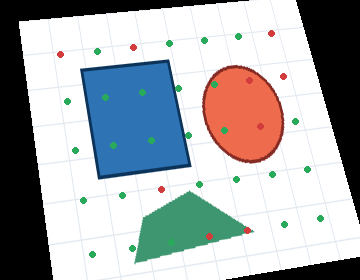
\includegraphics[width=0.82\textwidth]{artifacts/registration_ransac_overlay.png}
  \caption{RANSAC配准结果示意：绿色为内点投影，红色为被剔除的离群匹配}
  \label{fig:ransac}
\end{figure}

\subsection{实验二：扰动下的分割稳定性}
第二个实验把同一合成场景转换为不同扰动版本，包括低照度、高斯噪声和模糊。脚本用一个简单的颜色差异规则得到前景掩码，并计算与参考掩码的IoU。该实验有意使用简单算法，而不是直接调用大型分割模型，目的是把“鲁棒性评价”的概念讲清楚：同一任务在不同输入条件下应分别报告指标，而不是只展示一张成功样例。

本次实验中，clean、low\_light、gaussian\_noise三种条件的IoU均为1.000，blur条件下降到约0.979。这个结果说明当前规则对亮度变化和中等噪声较稳定，但模糊会带来轻微边界损伤。若换成\model{SAM 2}或其他提示式分割模型，同样可以保留这一评价框架：固定提示点或提示框，对扰动图像分别计算IoU、边界误差和运行时间，再分析失败样本。换言之，实验框架比具体模型更重要。

\begin{figure}[H]
  \centering
  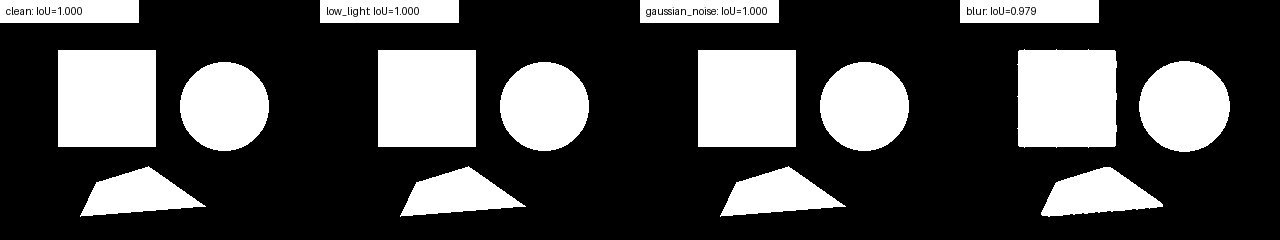
\includegraphics[width=\textwidth]{artifacts/robustness_masks.png}
  \caption{不同扰动条件下的掩码结果与IoU：鲁棒性评价应覆盖输入质量变化}
  \label{fig:robustness}
\end{figure}

\begin{table}[H]
\centering
\small
\caption{可复现实验结果摘要}
\begin{tabularx}{\textwidth}{C{3.2cm}Y Y}
\toprule
\textbf{实验项} & \textbf{结果} & \textbf{解释} \\
\midrule
RANSAC内点数 & 26/35 & 在含8个离群匹配的情况下，仍能找到主要几何一致点集 \\
中位重投影误差 & 1.13像素 & 配准精度处于像素级，说明估计的单应矩阵较接近真实变换 \\
角点迁移误差 & 1.04像素 & 对图像整体几何位置的恢复较稳定 \\
扰动掩码IoU & 1.000/1.000/1.000/0.979 & 低照度和噪声影响较小，模糊会带来轻微边界损伤 \\
\bottomrule
\end{tabularx}
\end{table}

\subsection{实验对前沿模型评价的启示}
这个小实验虽然简单，却能引出评价前沿视觉模型的三个原则。第一，必须固定输入、参数和随机种子，保证结果可复现。第二，必须报告失败条件，而不是只展示成功图。第三，必须把指标和任务意义对应起来：重投影误差关系到几何对齐，IoU关系到掩码可用性，运行时间关系到部署成本，人工复核率关系到系统负担。将来若进一步接入\model{DINOv2}特征、\model{SAM 2}分割或视觉语言模型问答，只需替换模型模块，评价闭环仍然成立。

\section{技术治理与社会责任：价值导向、责任边界与科技自立自强}
计算机视觉的最新进展不仅是算法问题，也关系到国家科技竞争力、数字经济发展和社会治理。《新一代人工智能发展规划》提出要把人工智能作为推动科技跨越发展、产业优化升级和生产力整体跃升的重要战略技术\cite{aiplan}。视觉基础模型、三维重建和具身智能正是人工智能从互联网应用走向实体经济的重要接口：它们让机器能够感知生产线、交通道路、农田矿山和医疗影像。学习这些技术，不应停留在调用模型接口，而应理解数据、算法、算力和应用场景之间的系统关系，增强科技自立自强意识。

同时，技术越强，责任边界越重要。生成式视觉能够降低创作门槛，也可能被用于深度伪造、谣言传播和侵犯肖像权；视觉监控能够提升公共安全，也可能造成过度采集和算法歧视；视觉语言模型能提升服务效率，也可能在关键场景中给出不可靠建议。《生成式人工智能服务管理暂行办法》强调生成式人工智能服务应遵守法律法规、尊重社会公德伦理、保护个人信息和知识产权\cite{genai2023}。这提示我们，算法研究必须与数据治理、安全评估、可解释性和责任追溯同步推进。

从青年学生角度看，思政要求不是在技术报告末尾附加口号，而是贯穿问题选择、方法设计和应用落地。在选择研究方向时，应关注服务国家重大需求和人民生活质量的视觉任务，例如智能制造、智慧医疗、灾害监测、无障碍辅助和文化遗产保护。在设计系统时，应坚持以人为本，把人的安全、尊严、隐私和知情权放在效率之前。在评价成果时，应同时看精度、鲁棒性、公平性、能耗和社会影响。只有这样，计算机视觉的最新进展才能真正转化为可信、可控、可持续的生产力。

\subsection{科技自立自强：从调用接口到掌握底层能力}
计算机视觉基础模型的竞争，本质上是数据、算法、算力和应用生态的综合竞争。如果只停留在调用国外闭源模型接口，短期可以获得演示效果，但长期会在数据安全、成本、可控性和产业升级方面受制于人。科技自立自强并不是排斥国际合作，而是要求我们理解核心原理、掌握关键工具、建设开放可复现的研究环境，并在国家重大需求场景中形成自己的数据与模型能力。

对学生而言，这意味着课程学习不能只满足于“会跑demo”。应进一步追问：模型训练数据来自哪里？是否能在本地部署？如何进行微调和评估？如果模型输出错误，能否定位原因？如果应用场景涉及中文文档、国产设备、地方产业和公共服务，模型是否真正适配？这些问题把个人学习与国家科技能力建设连接起来，也让课程报告具有更现实的价值。

\subsection{数据治理：尊重隐私、版权与公共利益}
视觉数据往往包含人脸、车牌、地理位置、医疗影像、工作场所和家庭环境，比普通文本数据更容易触及隐私和安全边界。训练和使用视觉模型时，必须明确数据来源、授权范围、脱敏方式和保存周期。生成式视觉还涉及版权和肖像权问题：模型可能学习艺术风格、复制人物形象，甚至生成误导性内容。因此，数据治理不是行政附属流程，而是视觉技术能否被社会信任的前提。

在报告所讨论的多个场景中，治理要求各不相同。医疗影像要重视患者隐私和医生责任，交通监控要防止过度采集和用途扩张，教育材料要标注AI生成内容，文化遗产数字化要尊重文物真实性和版权归属。技术人员应在系统设计阶段就考虑这些问题，例如加入权限控制、日志审计、水印标识、数据最小化和人工复核，而不是等到问题发生后再补救。

\subsection{智能向善：把安全边界写进系统设计}
智能向善不是要求技术停止发展，而是要求技术发展始终服务人的福祉。视觉基础模型可以提升生产效率，也可能带来监控滥用；生成式视频可以服务创作教育，也可能制造虚假信息；VLA和世界模型可以推动机器人应用，也可能在安全约束不足时造成现实伤害。因此，先进视觉系统应把安全边界写进设计：高风险场景保留人工确认，模型输出附带不确定性提示，生成内容带有来源标识，机器人动作经过约束检查。

这也要求评价体系从单一精度转向综合责任。一个模型如果在公开榜单上精度高，却在特定人群、弱光环境或罕见场景中系统性失误，就不能称为真正可靠。一个生成模型如果画面质量高，却无法防止深度伪造滥用，也不能只以“技术先进”为理由忽视风险。课程报告选择在技术综述中加入治理和伦理分析，正是为了体现工程教育中的责任意识。

\subsection{青年工程人才的使命}
作为学习计算机视觉的学生，我们面对的是一个快速变化的领域。模型会更新，榜单会变化，但工程判断、科学精神和社会责任不会过时。未来无论从事算法研究、软件开发、产品设计还是行业应用，都应坚持三个原则：第一，尊重事实，用可复现实验和数据支撑判断；第二，尊重边界，在高风险场景中保持谨慎；第三，服务需求，把技术能力用于解决真实问题。只有把专业能力与价值判断结合起来，才能让计算机视觉成为推动社会进步的可靠力量。

\section{展望}
第一，视觉模型会继续向统一多模态模型演进。未来模型可能同时处理图像、视频、音频、三维场景、传感器数据和机器人动作，并通过统一接口完成观察、理解、生成和控制。第二，长视频和长期记忆会成为关键能力。真实任务往往持续数分钟甚至数小时，模型需要记住目标、环境变化和任务进度，而不是只理解单帧图像。第三，三维和物理一致性会重新获得重要地位。生成式模型若要服务自动驾驶、机器人和工业仿真，就必须接受几何约束、动力学约束和可验证评估。

第四，高效部署会成为基础研究的重要指标。边缘设备、移动终端和机器人无法承受无限算力，动态计算、模型蒸馏、量化和小模型迁移将持续发展。第五，可信治理会从外部约束变成模型设计的一部分。未来视觉系统需要内置水印、数据来源记录、不确定性估计、拒答机制和审计接口。第六，开源生态和国产模型会更加重要。只有在可复现、可审计、可本地化部署的生态中，视觉算法才能更好服务教育、科研和产业升级。

从2026年前后的公开进展看，实时视频感知会成为下一阶段重点。\model{SAM 3.1}等工作把检测、分割、跟踪和文本提示进一步结合，强调实时视频中的多目标推理与可访问性\cite{sam31}。这意味着未来分割模型不再只是离线标注工具，而可能成为视频编辑、机器人观察、安防巡检和AR交互中的基础组件。随之而来的挑战是多目标长期跟踪、提示冲突处理、视频内存管理和实时部署成本。

世界模型也会继续向可交互、可控制和可验证方向发展。\model{Genie 3}被定位为新的世界模型前沿，展示了从提示生成可交互环境的可能性\cite{genie3}。但未来真正重要的问题不是“能否生成更逼真的世界”，而是“这个世界能否支持可靠学习和安全决策”。如果生成环境与真实世界差异过大，智能体可能在虚拟环境中学到错误策略。因此，世界模型需要与真实数据、物理约束、任务评价和人类反馈结合，逐步从视觉演示走向可验证仿真。

另一个趋势是模型能力的模块化与本地化。大型闭源多模态模型在综合能力上很强，但教育、医疗、工业和政务场景常常需要本地部署、数据不出域和可审计流程。未来可能出现更多“通用底座 + 行业适配 + 轻量边缘模型”的组合：云端模型负责复杂推理，本地模型负责实时感知和隐私敏感任务，行业知识库负责标准和流程约束。这种架构对学生提出了更高要求：既要理解基础模型，也要理解系统工程、数据治理和部署优化。

最后，评价体系会成为决定视觉技术能否进入关键领域的核心。未来高水平论文和工程系统不应只报告平均精度，还应报告跨域鲁棒性、失败案例、能耗、延迟、隐私风险、生成内容标识和人工接管机制。对于课程学习而言，最值得培养的能力就是把新模型放进完整系统中审视：它解决了什么问题，依赖什么假设，在哪些场景会失败，如何被验证，如何被负责任地使用。

\section{报告总结}
本文围绕“介绍算法与技术的最新进展”这一主题，梳理了2023—2026年计算机视觉从基础表征到世界模型的主要变化。总体来看，最新进展可以概括为三句话：第一，视觉模型正在基础模型化，分割、检测、描述和几何估计逐渐统一到可提示、可迁移的框架中；第二，视觉语言模型和生成式视频模型正在把视觉系统从静态识别推向多模态推理、内容生成和世界模拟；第三，三维视觉和具身智能正在把视觉能力连接到物理行动，使“看见”最终服务“理解、预测和执行”。报告还通过一个可复现实验展示了RANSAC配准、扰动鲁棒性和指标分析，说明课程基础知识仍然是理解前沿模型可靠性的关键。

这些进展令人振奋，但也提醒我们不能把算法能力等同于社会价值。优秀的计算机视觉系统既要有高精度和高效率，也要有安全边界、数据合规、可解释机制和面向真实需求的应用设计。对学生而言，学习最新算法的意义不仅是掌握模型名称和论文结论，更是理解技术演进背后的科学问题、工程约束和价值责任。只有把专业学习、国家需求和社会责任结合起来，才能让计算机视觉技术在未来真正发挥积极作用。

\newpage
\begin{thebibliography}{99}
\addcontentsline{toc}{section}{参考文献}
\bibitem{dinov2} Oquab M, Darcet T, Moutakanni T, et al. DINOv2: Learning Robust Visual Features without Supervision[EB/OL]. arXiv:2304.07193, 2023. \url{https://arxiv.org/abs/2304.07193}
\bibitem{sam2} Ravi N, Gabeur V, Hu Y T, et al. SAM 2: Segment Anything in Images and Videos[EB/OL]. arXiv:2408.00714, 2024. \url{https://arxiv.org/abs/2408.00714}
\bibitem{florence2} Xiao B, Wu H, Xu W, et al. Florence-2: Advancing a Unified Representation for a Variety of Vision Tasks[EB/OL]. arXiv:2311.06242, 2023. \url{https://arxiv.org/abs/2311.06242}
\bibitem{yoloworld} Cheng T, Song L, Ge Y, et al. YOLO-World: Real-Time Open-Vocabulary Object Detection[EB/OL]. arXiv:2401.17270, 2024. \url{https://arxiv.org/abs/2401.17270}
\bibitem{qwen2vl} Wang P, Bai S, Tan S, et al. Qwen2-VL: Enhancing Vision-Language Model's Perception of the World at Any Resolution[EB/OL]. arXiv:2409.12191, 2024. \url{https://arxiv.org/abs/2409.12191}
\bibitem{qwen25vl} Bai S, Chen K, Liu X, et al. Qwen2.5-VL Technical Report[EB/OL]. arXiv:2502.13923, 2025. \url{https://arxiv.org/abs/2502.13923}
\bibitem{gemini15} Gemini Team, Georgiev P, Lei V I, et al. Gemini 1.5: Unlocking Multimodal Understanding across Millions of Tokens of Context[EB/OL]. arXiv:2403.05530, 2024. \url{https://arxiv.org/abs/2403.05530}
\bibitem{gpt4o} OpenAI. GPT-4o System Card[EB/OL]. 2024. \url{https://openai.com/index/gpt-4o-system-card/}
\bibitem{llavaov} Li B, Zhang Y, Guo D, et al. LLaVA-OneVision: Easy Visual Task Transfer[EB/OL]. arXiv:2408.03326, 2024. \url{https://arxiv.org/abs/2408.03326}
\bibitem{depthanythingv2} Yang L, Kang B, Huang Z, et al. Depth Anything V2[EB/OL]. arXiv:2406.09414, 2024. \url{https://arxiv.org/abs/2406.09414}
\bibitem{vggt} Wang J, Chen M, Karaev N, et al. VGGT: Visual Geometry Grounded Transformer[EB/OL]. arXiv:2503.11651, 2025. \url{https://arxiv.org/abs/2503.11651}
\bibitem{gs3d} Kerbl B, Kopanas G, Leimkühler T, et al. 3D Gaussian Splatting for Real-Time Radiance Field Rendering[EB/OL]. arXiv:2308.04079, 2023. \url{https://arxiv.org/abs/2308.04079}
\bibitem{pixelsplat} Charatan D, Li S, Tagliasacchi A, et al. pixelSplat: 3D Gaussian Splats from Image Pairs for Scalable Generalizable 3D Reconstruction[EB/OL]. arXiv:2312.12337, 2023. \url{https://arxiv.org/abs/2312.12337}
\bibitem{sd3} Esser P, Kulal S, Blattmann A, et al. Scaling Rectified Flow Transformers for High-Resolution Image Synthesis[EB/OL]. arXiv:2403.03206, 2024. \url{https://arxiv.org/abs/2403.03206}
\bibitem{pixartdelta} Chen J, Wu Y, Luo S, et al. PIXART-$\delta$: Fast and Controllable Image Generation with Latent Consistency Models[EB/OL]. arXiv:2401.05252, 2024. \url{https://arxiv.org/abs/2401.05252}
\bibitem{dydit} Zhao W, Han Y, Tang J, et al. Dynamic Diffusion Transformer[EB/OL]. arXiv:2410.03456, 2024. \url{https://arxiv.org/abs/2410.03456}
\bibitem{sora} OpenAI. Video Generation Models as World Simulators[EB/OL]. 2024. \url{https://openai.com/index/video-generation-models-as-world-simulators/}
\bibitem{moviegen} Polyak A, Zohar A, Brown A, et al. Movie Gen: A Cast of Media Foundation Models[EB/OL]. arXiv:2410.13720, 2024. \url{https://arxiv.org/abs/2410.13720}
\bibitem{veo} Google DeepMind. Veo 3.1[EB/OL]. \url{https://deepmind.google/models/veo/}
\bibitem{genie2} Google DeepMind. Genie 2: A Large-Scale Foundation World Model[EB/OL]. 2024. \url{https://deepmind.google/blog/genie-2-a-large-scale-foundation-world-model/}
\bibitem{openvla} Kim M J, Pertsch K, Karamcheti S, et al. OpenVLA: An Open-Source Vision-Language-Action Model[EB/OL]. arXiv:2406.09246, 2024. \url{https://arxiv.org/abs/2406.09246}
\bibitem{pi0} Black K, Brown N, Driess D, et al. $\pi_0$: A Vision-Language-Action Flow Model for General Robot Control[EB/OL]. arXiv:2410.24164, 2024. \url{https://arxiv.org/abs/2410.24164}
\bibitem{paligemma2} Beyer L, Steiner A, Pinto A S, et al. PaliGemma 2: A Family of Versatile VLMs for Transfer[EB/OL]. arXiv:2412.03555, 2024. \url{https://arxiv.org/abs/2412.03555}
\bibitem{idefics2} Lauren{\c c}on H, Tronchon L, Cord M, et al. What Matters when Building Vision-Language Models?[EB/OL]. arXiv:2405.02246, 2024. \url{https://arxiv.org/abs/2405.02246}
\bibitem{vjepa2} Assran M, Bardes A, Fan D, et al. V-JEPA 2: Self-Supervised Video Models Enable Understanding, Prediction and Planning[EB/OL]. arXiv:2506.09985, 2025. \url{https://arxiv.org/abs/2506.09985}
\bibitem{sam} Kirillov A, Mintun E, Ravi N, et al. Segment Anything[EB/OL]. arXiv:2304.02643, 2023. \url{https://arxiv.org/abs/2304.02643}
\bibitem{dinov3} Sim{\'e}oni O, Vo H V, Seitzer M, et al. DINOv3[EB/OL]. arXiv:2508.10104, 2025. \url{https://arxiv.org/abs/2508.10104}
\bibitem{siglip2} Tschannen M, Gritsenko A, Wang X, et al. SigLIP 2: Multilingual Vision-Language Encoders with Improved Semantic Understanding, Localization, and Dense Features[EB/OL]. arXiv:2502.14786, 2025. \url{https://arxiv.org/abs/2502.14786}
\bibitem{svd} Blattmann A, Dockhorn T, Kulal S, et al. Stable Video Diffusion: Scaling Latent Video Diffusion Models to Large Datasets[EB/OL]. arXiv:2311.15127, 2023. \url{https://arxiv.org/abs/2311.15127}
\bibitem{lumiere} Bar-Tal O, Chefer H, Tov O, et al. Lumiere: A Space-Time Diffusion Model for Video Generation[EB/OL]. arXiv:2401.12945, 2024. \url{https://arxiv.org/abs/2401.12945}
\bibitem{sora2} OpenAI. Sora 2 System Card[EB/OL]. 2025. \url{https://openai.com/index/sora-2-system-card/}
\bibitem{zipnerf} Barron J T, Mildenhall B, Verbin D, et al. Zip-NeRF: Anti-Aliased Grid-Based Neural Radiance Fields[EB/OL]. arXiv:2304.06706, 2023. \url{https://arxiv.org/abs/2304.06706}
\bibitem{gsslam} Yan C, Qu D, Wang D, et al. GS-SLAM: Dense Visual SLAM with 3D Gaussian Splatting[EB/OL]. arXiv:2311.11700, 2023. \url{https://arxiv.org/abs/2311.11700}
\bibitem{rt2} Brohan A, Brown N, Carbajal J, et al. RT-2: Vision-Language-Action Models Transfer Web Knowledge to Robotic Control[EB/OL]. arXiv:2307.15818, 2023. \url{https://arxiv.org/abs/2307.15818}
\bibitem{dreamerv3} Hafner D, Pasukonis J, Ba J, et al. Mastering Diverse Domains through World Models[EB/OL]. arXiv:2301.04104, 2023. \url{https://arxiv.org/abs/2301.04104}
\bibitem{genie} Bruce J, Dennis M, Edwards A, et al. Genie: Generative Interactive Environments[EB/OL]. Google DeepMind, 2024. \url{https://deepmind.google/research/publications/60474/}
\bibitem{genie3} Google DeepMind. Genie 3: A New Frontier for World Models[EB/OL]. 2025. \url{https://deepmind.google/blog/genie-3-a-new-frontier-for-world-models/}
\bibitem{sam31} Meta AI. SAM 3.1: Faster and More Accessible Real-Time Video Detection and Tracking with Multiplexing and Global Reasoning[EB/OL]. 2026. \url{https://ai.meta.com/blog/segment-anything-model-3/}
\bibitem{aiplan} 国务院. 国务院关于印发新一代人工智能发展规划的通知[EB/OL]. 2017. \url{https://www.gov.cn/zhengce/content/2017-07/20/content_5211996.htm}
\bibitem{genai2023} 国家互联网信息办公室等. 生成式人工智能服务管理暂行办法[EB/OL]. 2023. \url{https://www.cac.gov.cn/2023-07/13/c_1690898327029107.htm}
\end{thebibliography}

\end{document}
